\documentclass{beamer}
\usepackage[utf8]{inputenc}
\usepackage[utf8]{vietnam}
\usepackage{utopia} %font utopia imported
\usepackage{graphicx} % Allows including images
\usepackage{booktabs} % Allows the use of \toprule, \midrule and \bottomrule in tables
\usepackage[vietnamese]{babel}

\usetheme{Madrid}
\usecolortheme{default}

%------------------------------------------------------------
%This block of code defines the information to appear in the
%Title page
\graphicspath{ {./images/} }
\title[React Native] %optional
{Tìm hiểu về React Native và \\ Xây dựng ứng dụng minh họa}

\subtitle{Môn: Phát triễn ứng dụng di động}

\author[A.Duy, B.Duy, H.Như] % (optional)
{Phạm Anh Duy - 51702088 \\ Trần Ngọc Bảo Duy - 51702091 \\ Trương Thị Huỳnh Như - 51702154 }

\institute[TDTU] % (optional)
{
  Khoa Công nghệ thông tin\\
  Trường Đại học Tôn Đức Thắng
}

\logo{
\includegraphics[height=1cm]{TDTU_logo.png}}

\date[TpHCM 2020] % (optional)
{{Thành phố Hồ Chí Minh, 2020}}


%End of title page configuration block
%------------------------------------------------------------



%------------------------------------------------------------
%The next block of commands puts the table of contents at the 
%beginning of each section and highlights the current section:

\AtBeginSection[]
{
  \begin{frame}
    \frametitle{Nội Dung Chính}
    \tableofcontents[currentsection]
  \end{frame}
}
%------------------------------------------------------------


\begin{document}

%The next statement creates the title page.
\frame{\titlepage}


%---------------------------------------------------------
%This block of code is for the table of contents after
%the title page
\begin{frame}
\frametitle{Nội Dung Chính}
\tableofcontents
\end{frame}
%---------------------------------------------------------



\section{Giới thiệu đề tài}

\begin{frame}
\frametitle{Giới thiệu đề tài}

Smartphone đã và đang trở nên rất phổ biến đối với tất cả mọi người. Và sử dụng smartphone như một thói quen hàng ngày và đã trở thành thứ không thể thiếu trong cuộc sống hiện đại ngày nay.

\begin{figure}[h]
	\vspace{5pt}
	\centering
	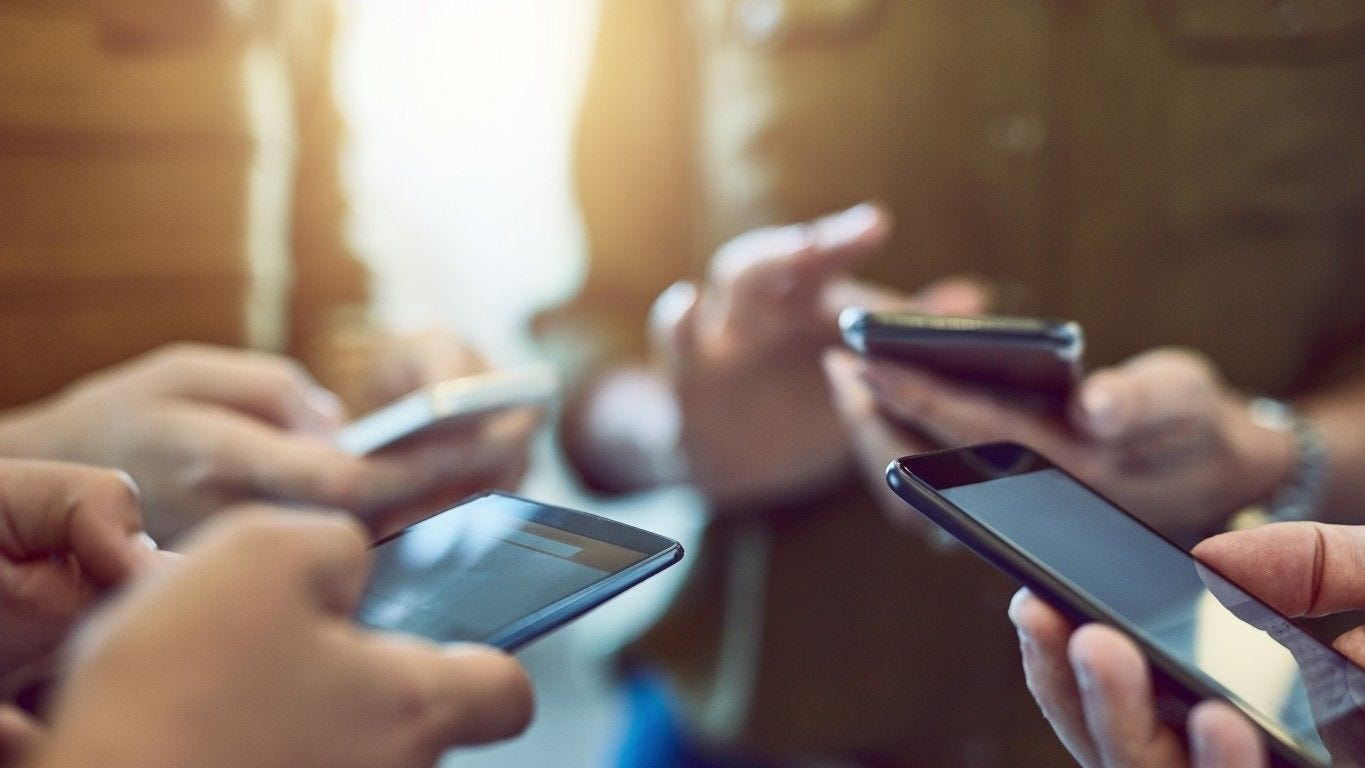
\includegraphics[width=0.6\textwidth]{use-smartphone}
\end{figure}

\end{frame}

\begin{frame}
\frametitle{Giới thiệu đề tài}

Nắm được nhu cầu đó, các hãng đã sản xuất ra nhiều mẫu mã điện thoại phù hợp với nhu cầu người dùng. Bên cạnh đó, để tạo ra một hệ sinh thái ưu việt hấp dẫn người dùng, các nhà phát triễn đã xây dựng và hoàn thiện nên các hệ điều hành của riêng mình nhằm tạo ra sự đa dạng, và nhiều sự lựa chọn cho người dùng. Nổi trội nhất là hai hệ điều hành: Android, iOS.

\begin{figure}[h]
	\vspace{5pt}
	\centering
	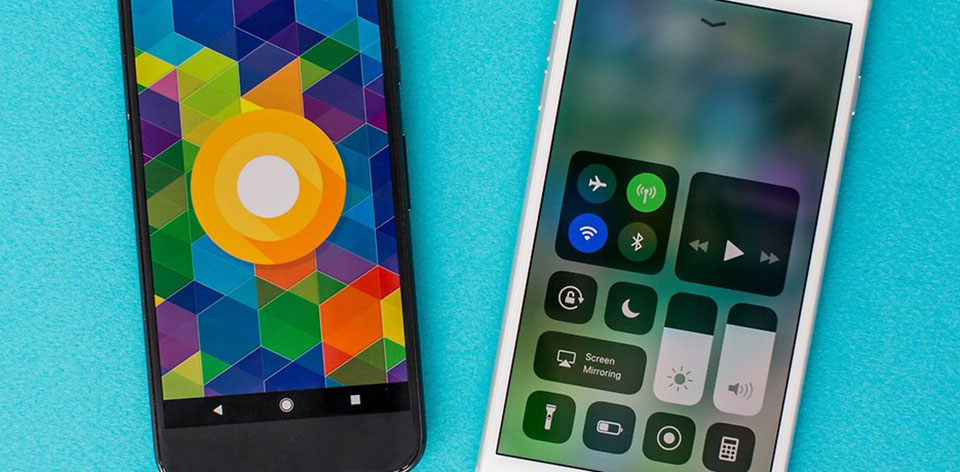
\includegraphics[width=0.6\textwidth]{android-ios}
\end{figure}

\end{frame}

\begin{frame}
\frametitle{Giới thiệu đề tài}

Trước đây, các nhà phát triễn muốn viết ứng dụng trên Andriod hay iOS đều phải sử dụng những ngôn ngữ lập trình riêng biệt, phù hợp với hệ điều hành. Ví dụ: Java để viết ứng dụng trên Android, Swift để viết ứng dụng trên iOS.

Liệu có thể nào dùng một ngôn ngữ lập trình mà có thể viết ứng dụng trên hai nền tảng ?

\end{frame}

\begin{frame}
\frametitle{Giới thiệu đề tài}

Hiện nay, với sự phát triễn của công nghệ, ta có thể viết được ứng trên trên hai nền tảng Android, iOS mà chỉ dùng một ngôn ngữ lập trình.

Đó chính là Javascript với sự hỗ trợ của framework React-Naitve.

\begin{figure}[h]
	\vspace{5pt}
	\centering
	
\includegraphics[width=0.6\textwidth]{react-native}
\end{figure}

\end{frame}



\section{Khái niệm về Native App, Mobile Web App và Hybrid App}

\begin{frame}
\label{NATIVE_APP}
\frametitle{Native App}

Native app hay còn gọi là ứng dụng gốc được viết cho một loại nền tảng như iOS, Android,...

\begin{columns}

\column{0.5\textwidth}
\begin{figure}[h]
	\vspace{5pt}
	\centering
	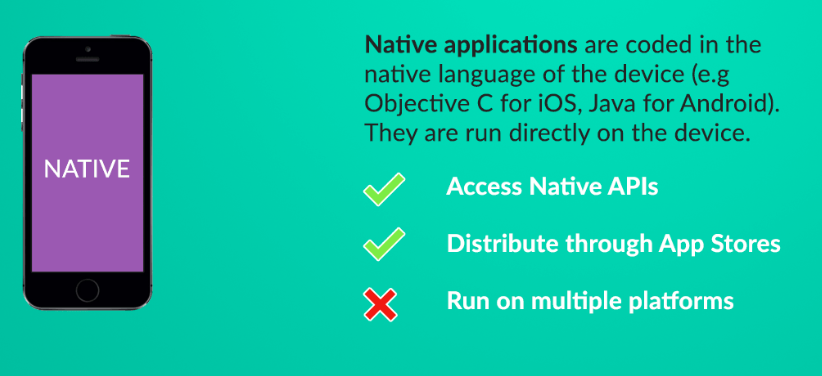
\includegraphics[width=.9\textwidth]{native-app-1}
\end{figure}


\column{0.5\textwidth}
\begin{figure}[h]
	\vspace{5pt}
	\centering
	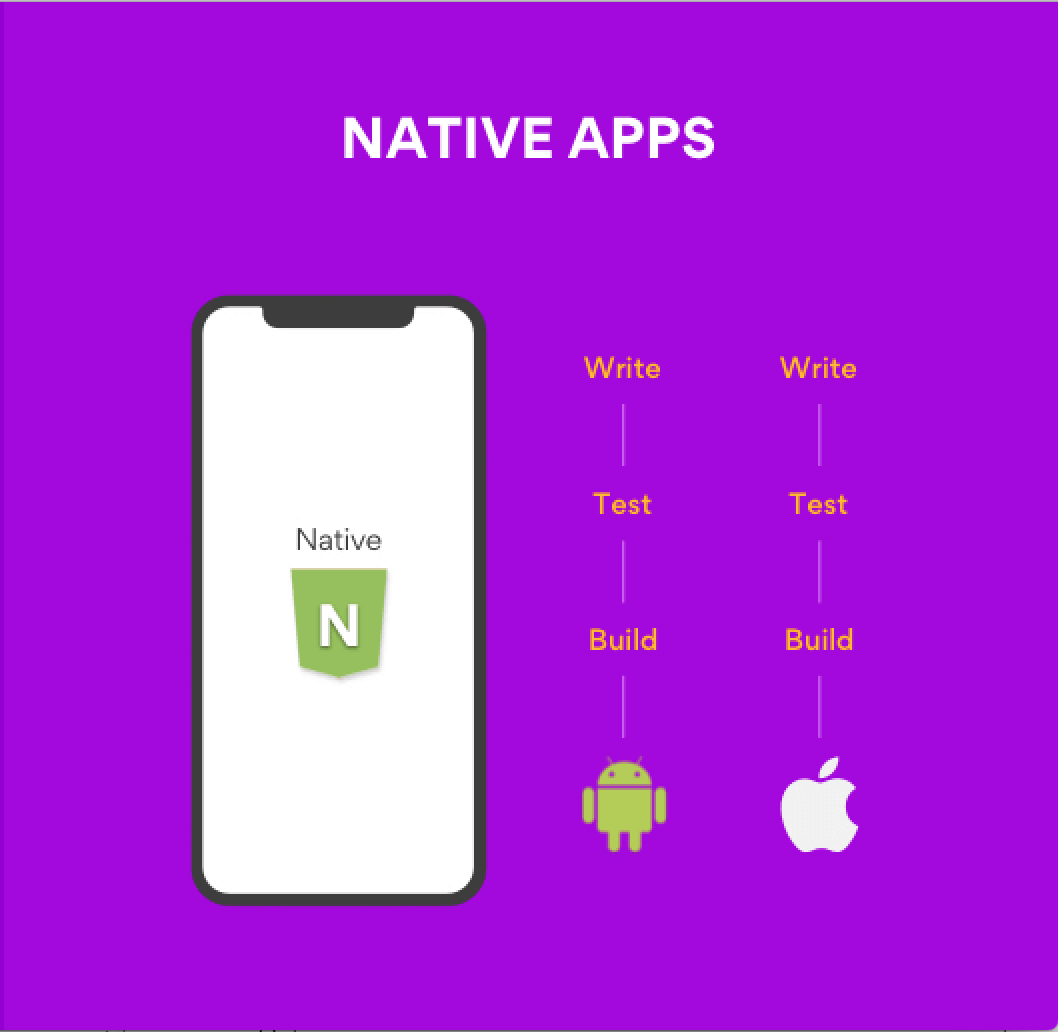
\includegraphics[width=0.7\textwidth]{native-app-2}
\end{figure}

\end{columns}

\end{frame}


\begin{frame}
\frametitle{Native App}

Ưu điểm:
\begin{itemize}
    \item<1-> Performance (Hiệu năng).
    \item<2-> Features (Các tính năng).
\end{itemize}

\end{frame}

\begin{frame}
\frametitle{Native App}

Nhược điểm:
\begin{itemize}
	\item<1-> Không thể cross platform.
	\item<2-> Tính nhất quán.
	\item<3-> Tính bảo trì, nâng cấp.
\end{itemize}

\end{frame}

\begin{frame}
\label{MOBILE_WEB_APP}
\frametitle{Mobile Web App}

Là ứng dụng chạy trên nền web, được viết bằng các ngôn ngữ web như HTML/CSS/JS jQuery và được tối ưu trên màn hình điện thoại.

\begin{figure}[h]
	\vspace{5pt}
	\centering
	
\includegraphics[width=0.7\textwidth]{mobile-web-app-1}
\end{figure}

\end{frame}


\begin{frame}
\frametitle{Mobile Web App}

Ưu điểm:
\begin{itemize}
    \item<1-> Cross platform.
    \item<2-> Dễ dàng phát triễn, nâng cấp hay sửa chữa.
    \item<3-> Thuận lợi cho việc SEO.
\end{itemize}

\end{frame}

\begin{frame}
\frametitle{Mobile Web App}

Nhược điểm:
\begin{itemize}
	\item<1-> Phải tối ưu cho các thiết bị di động riêng lẻ.
	\item<2-> Performance (Hiệu năng).
	\item<3-> Luôn phải chạy online.
\end{itemize}

\end{frame}


\begin{frame}
\frametitle{Hybrid App}

Là ứng dụng kết hợp những ưu điểm của cả \hyperlink{MOBILE_WEB_APP}{Mobile Web App} và \hyperlink{NATIVE_APP}{Native App}.

\begin{figure}[h]
	\vspace{5pt}
	\centering
	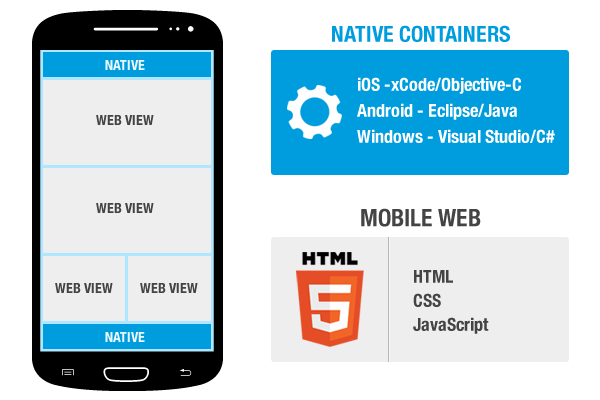
\includegraphics[width=0.6\textwidth]{Hybrid-App}
\end{figure}
\end{frame}


\begin{frame}
\frametitle{Hybrid App}

Ưu điểm:
\begin{itemize}
    \item<1-> Kết hợp được những điểm mạnh của \hyperlink{MOBILE_WEB_APP}{Mobile Web App} và \hyperlink{NATIVE_APP}{Native App}.
    \item<2-> Trải nghiệm cao.
\end{itemize}

\end{frame}


\section{React-Native}

\begin{frame}
\frametitle{Nguồn gốc}

\begin{itemize}
    \item<1-> Là framework do Facebook phát triễn.
    \item<2-> Build ứng dụng trên đa nền tảng.
\end{itemize}

\begin{figure}[h]
	\vspace{5pt}
	\centering
	
\includegraphics[width=0.6\textwidth]{react-native-2}
\end{figure}

\end{frame}

\begin{frame}
\frametitle{Ưu điểm}

\begin{itemize}
    \item<1-> Viết một lần dùng cho hai hệ điều hành.
    \item<2-> Khả năng reuse.
    \item<3-> Hot reloading.
    \item<4-> Cộng đồng phát triễn mạnh.
    \item<5-> ...
\end{itemize}

\end{frame}

\begin{frame}
\frametitle{Nhược điểm}

\begin{itemize}
    \item<1-> Vẫn cần phải biết native code.
    \item<2-> Hiệu năng thấp.
    \item<3-> Bảo mật chưa cao.
    \item<4-> Khả năng quản lý bộ nhớ.
\end{itemize}

\end{frame}


\section{Ứng dụng minh họa}

\begin{frame}
\frametitle{Ứng dụng học ngoại ngữ}

\begin{figure}[h]
	\centering
	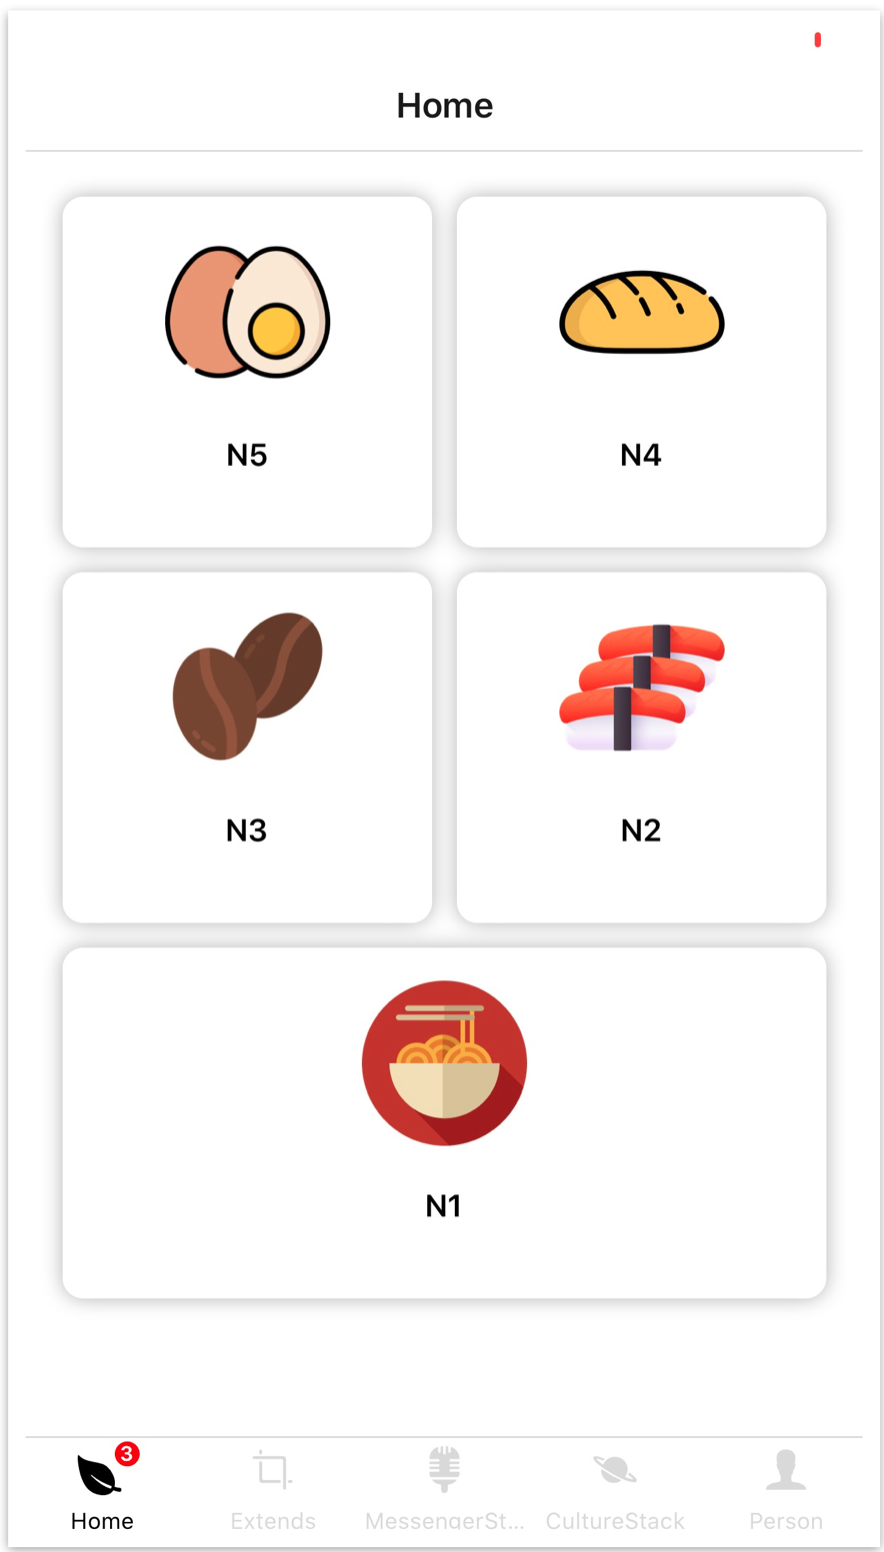
\includegraphics[width=.35\textwidth]{demo-1}
\end{figure}

\end{frame}

\begin{frame}
\frametitle{Ứng dụng học ngoại ngữ}

\begin{figure}[h]
	\centering
	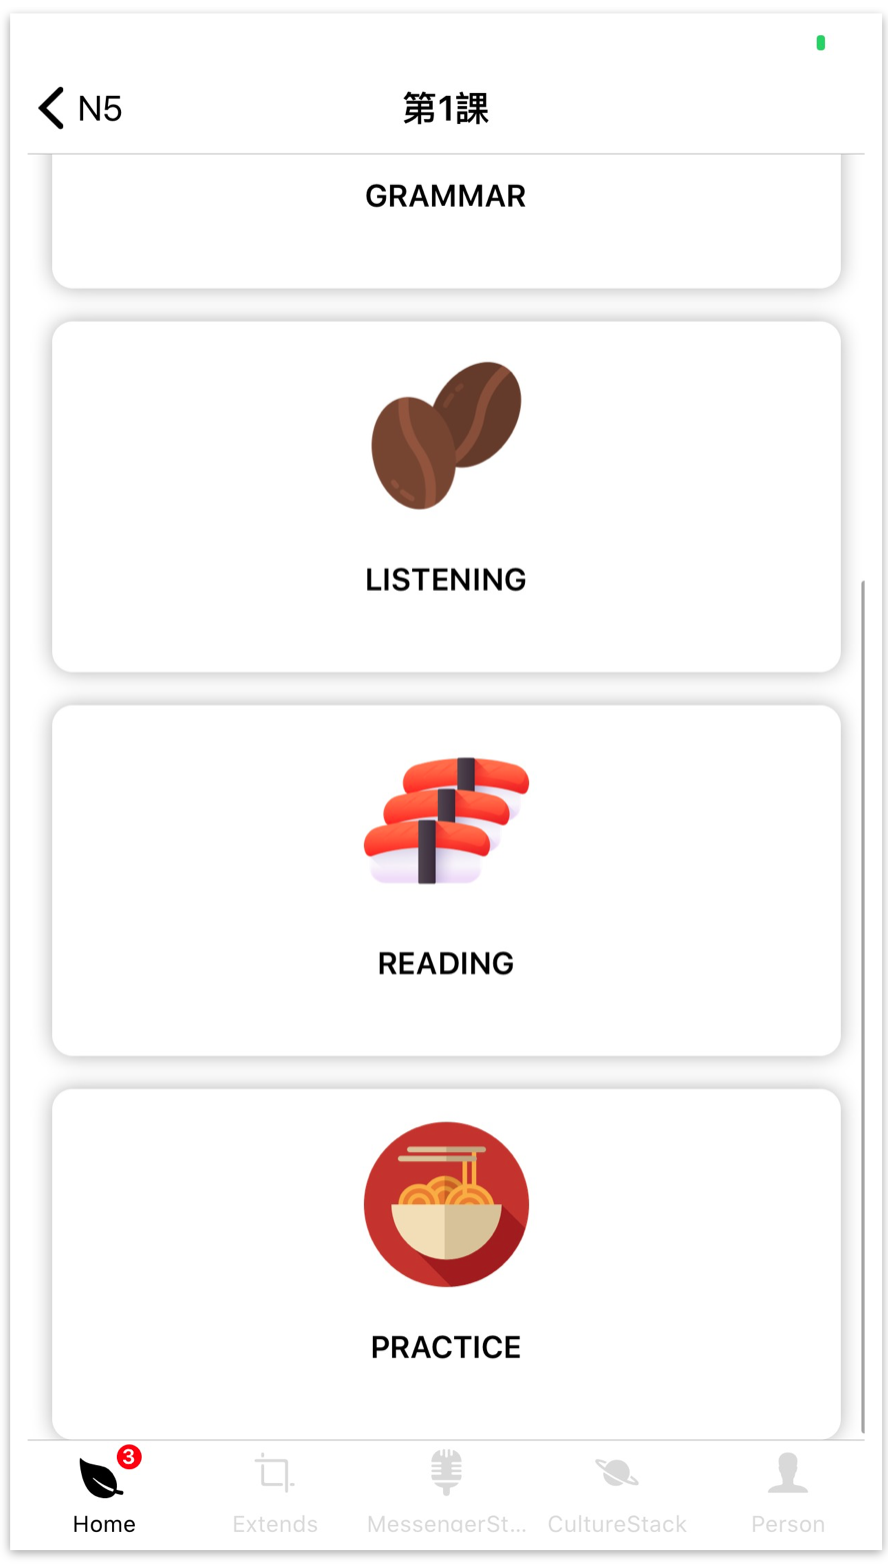
\includegraphics[width=.35\textwidth]{demo-2}
\end{figure}

\end{frame}

\begin{frame}
\frametitle{Ứng dụng học ngoại ngữ}

\begin{figure}[h]
	\centering
	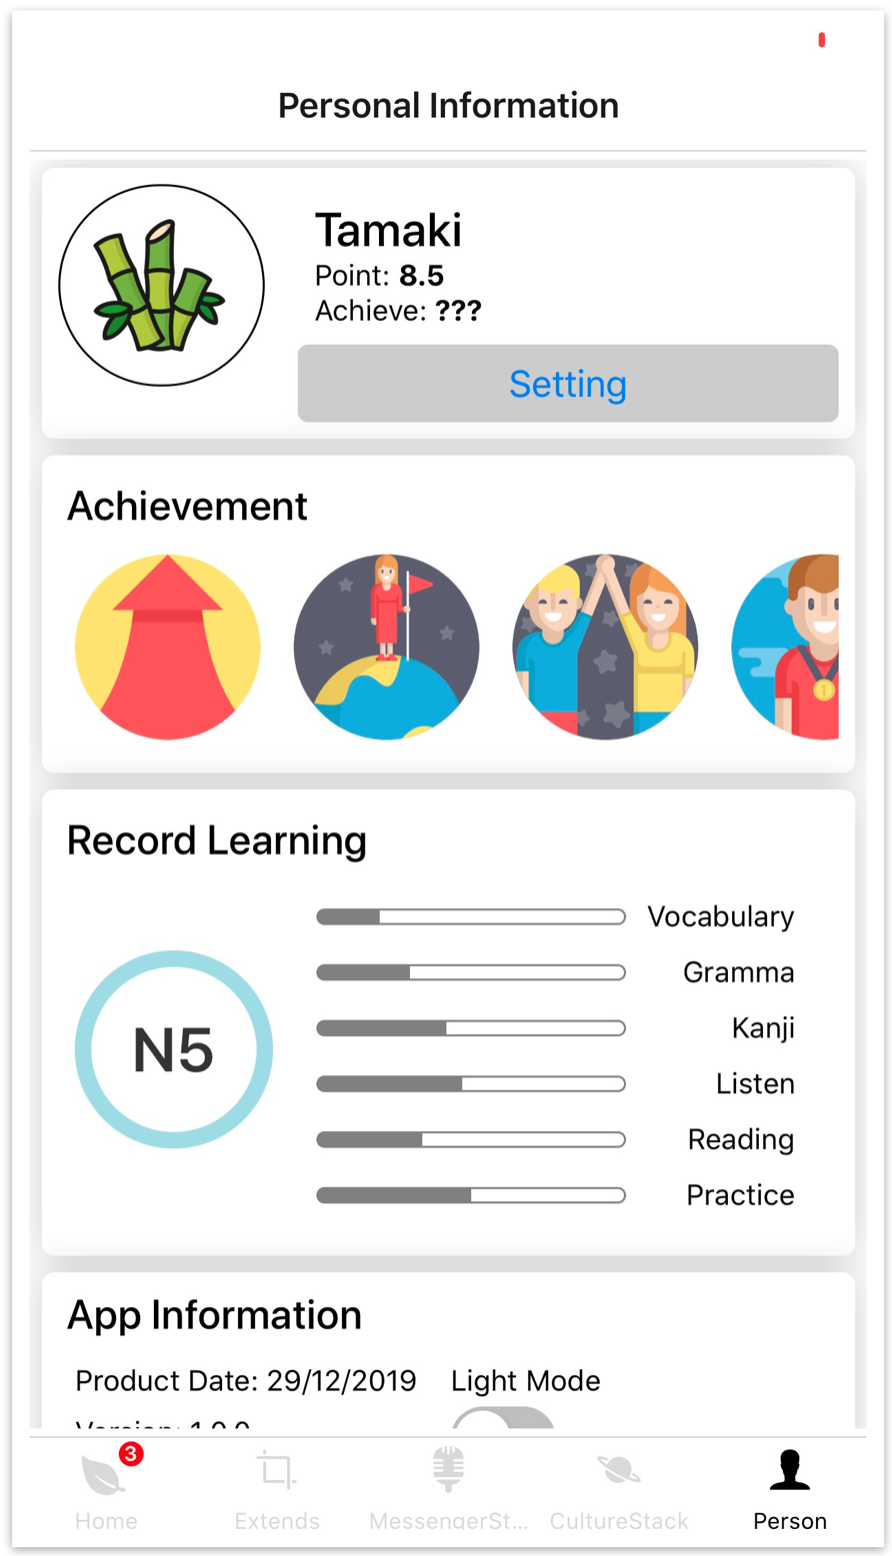
\includegraphics[width=.35\textwidth]{demo-3}
\end{figure}

\end{frame}

\begin{frame}
\frametitle{Ứng dụng học ngoại ngữ}

\begin{figure}[h]
	\centering
	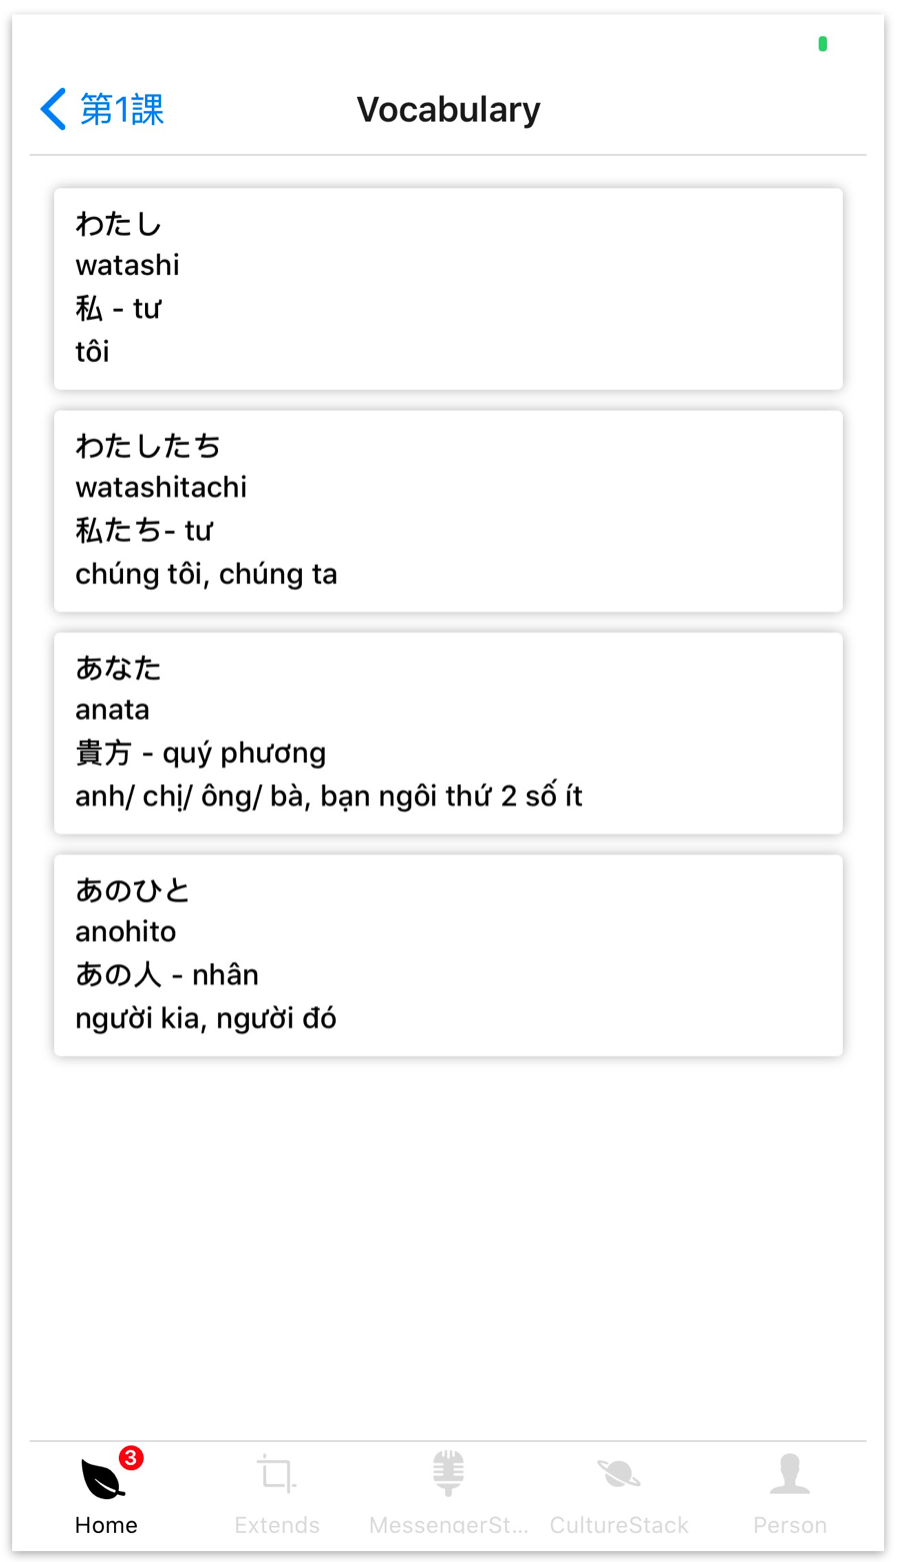
\includegraphics[width=.35\textwidth]{demo-4}
\end{figure}

\end{frame}

\begin{frame}
\frametitle{Ứng dụng học ngoại ngữ}

\begin{figure}[h]
	\centering
	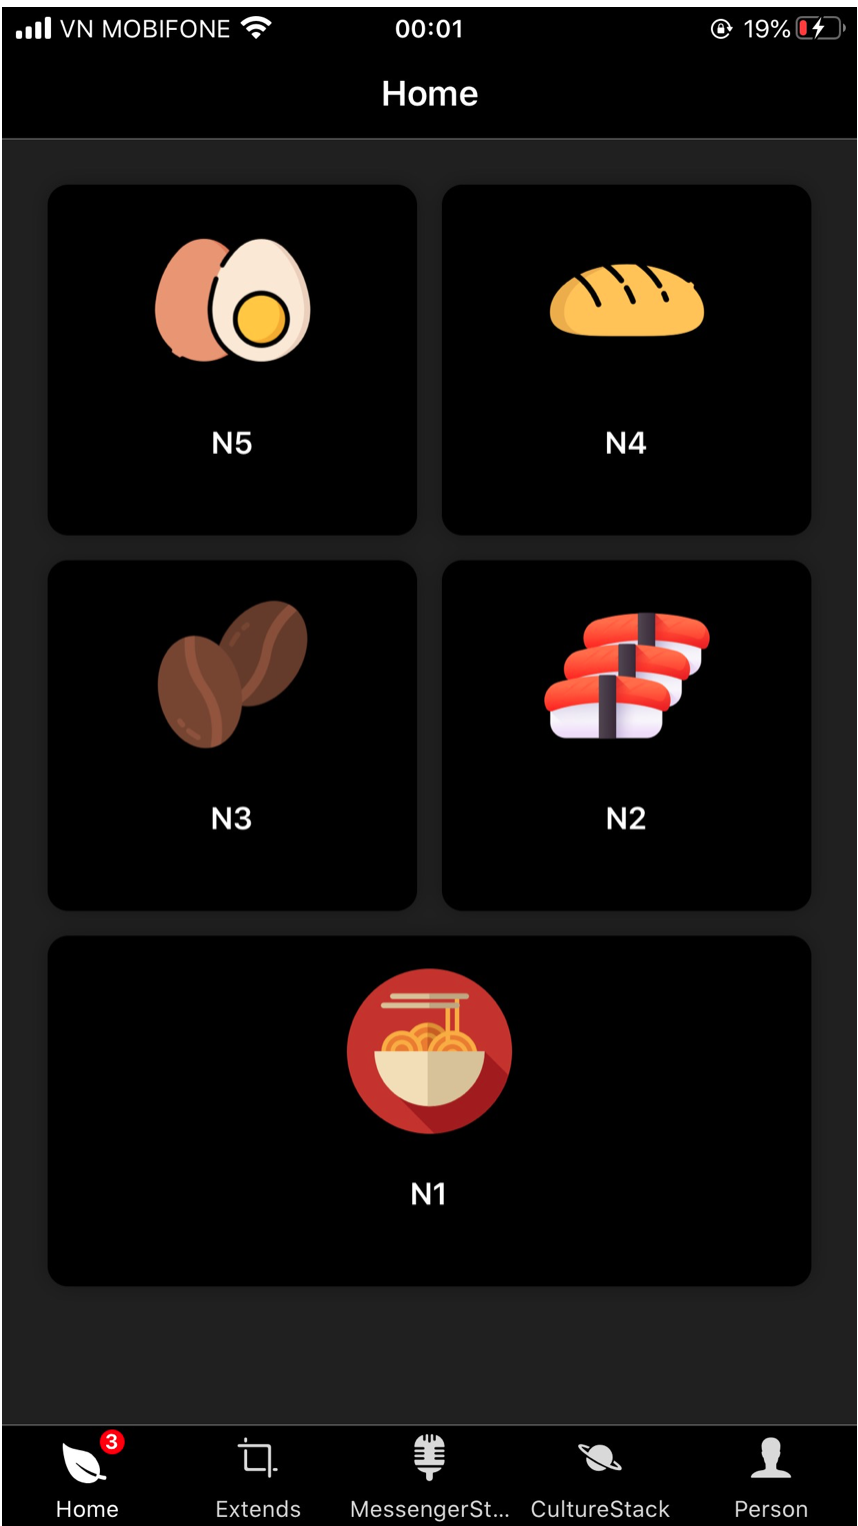
\includegraphics[width=.35\textwidth]{demo-5}
\end{figure}

\end{frame}

\begin{frame}
\frametitle{Ứng dụng học ngoại ngữ}

\begin{figure}[h]
	\centering
	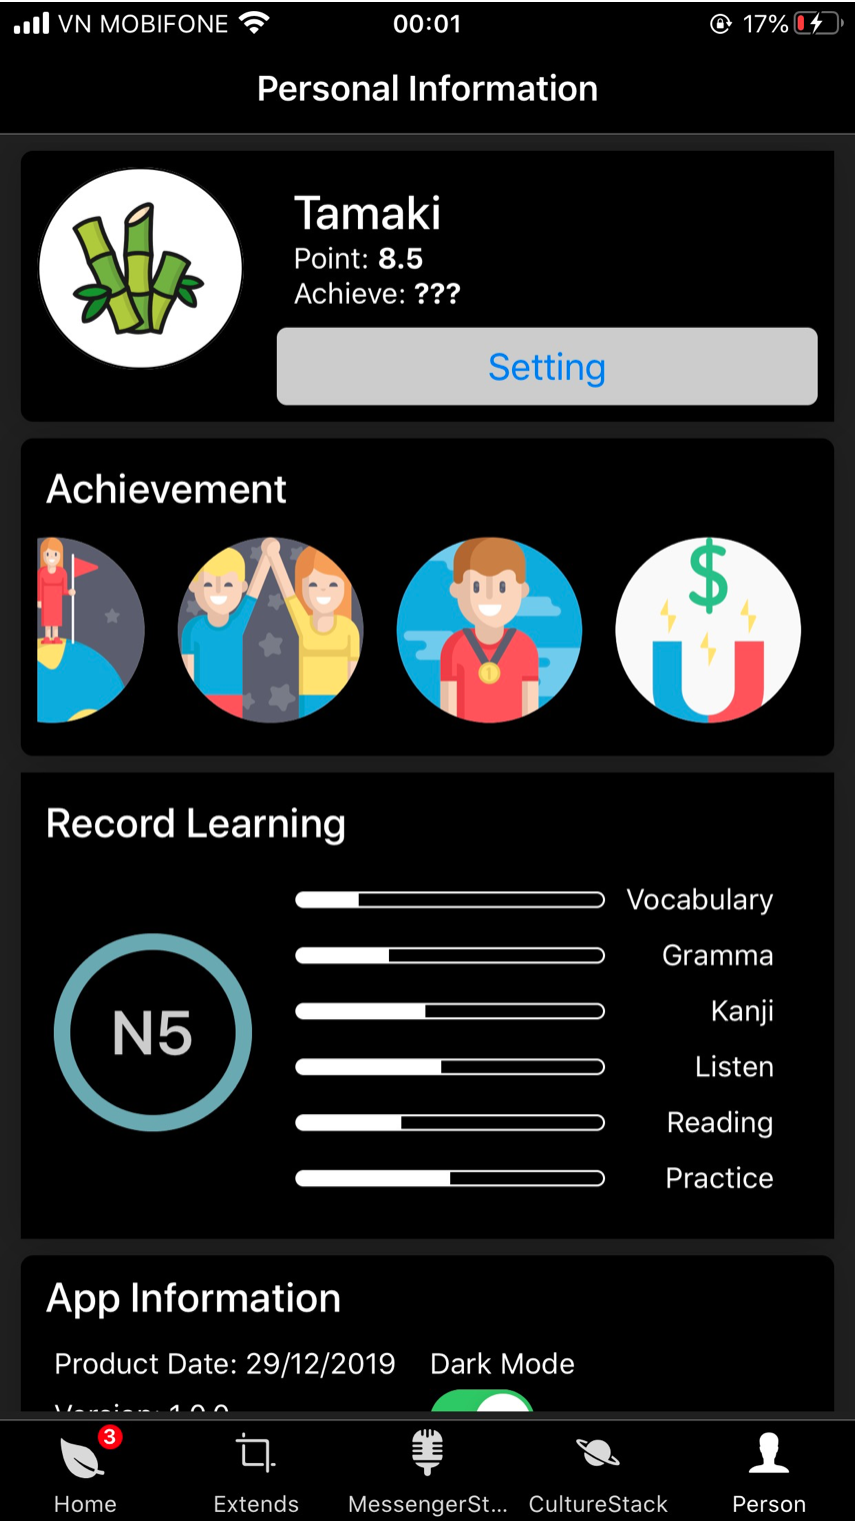
\includegraphics[width=.35\textwidth]{demo-6}
\end{figure}

\end{frame}

\begin{frame}
\frametitle{Ứng dụng học ngoại ngữ}

\begin{figure}[h]
	\centering
	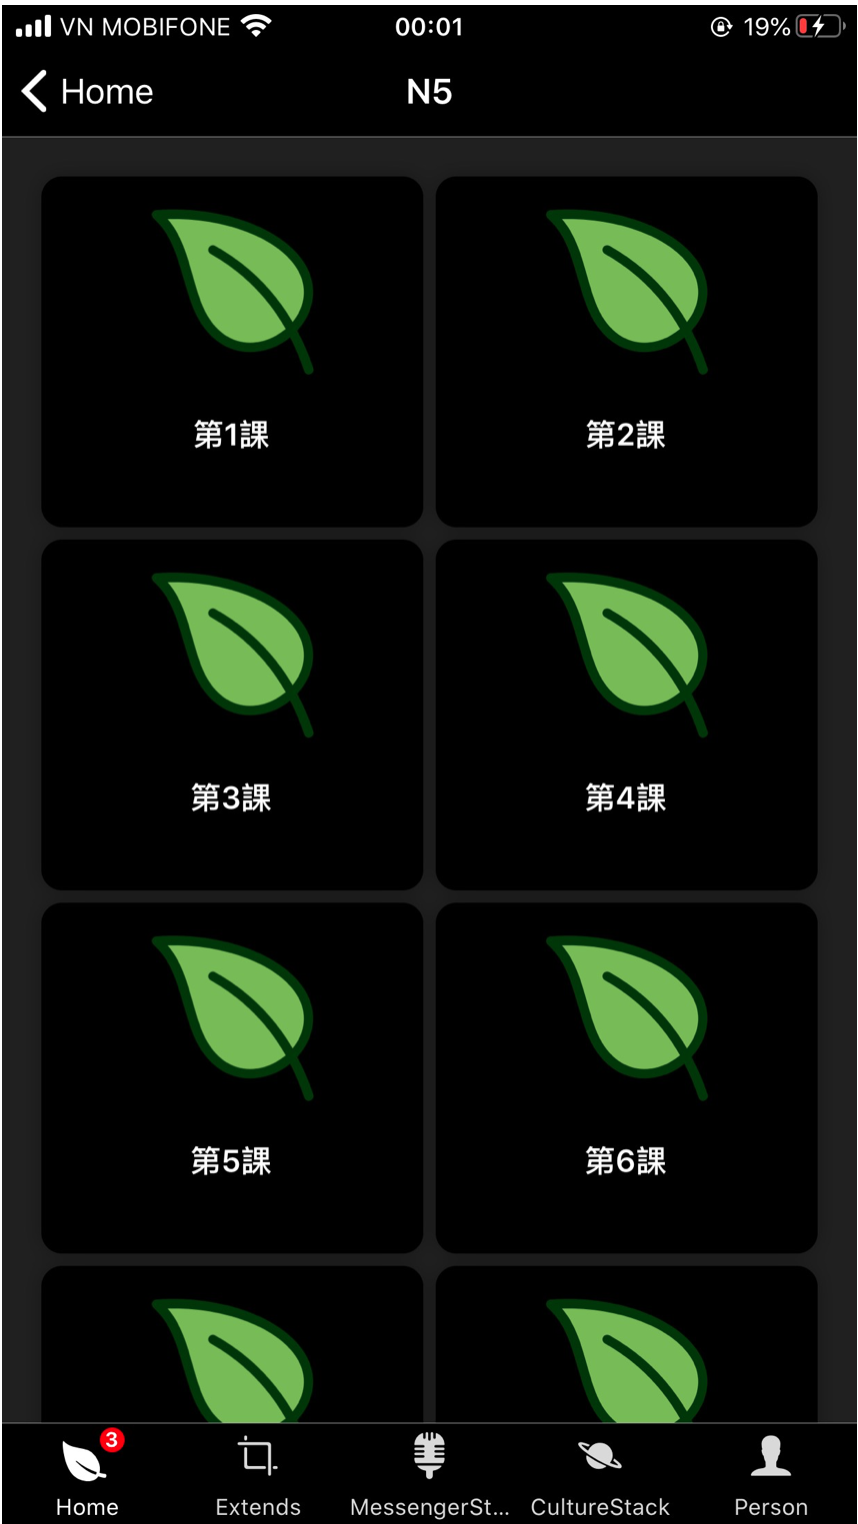
\includegraphics[width=.35\textwidth]{demo-7}
\end{figure}

\end{frame}

\begin{frame}
\frametitle{Ứng dụng học ngoại ngữ}

\begin{figure}[h]
	\centering
	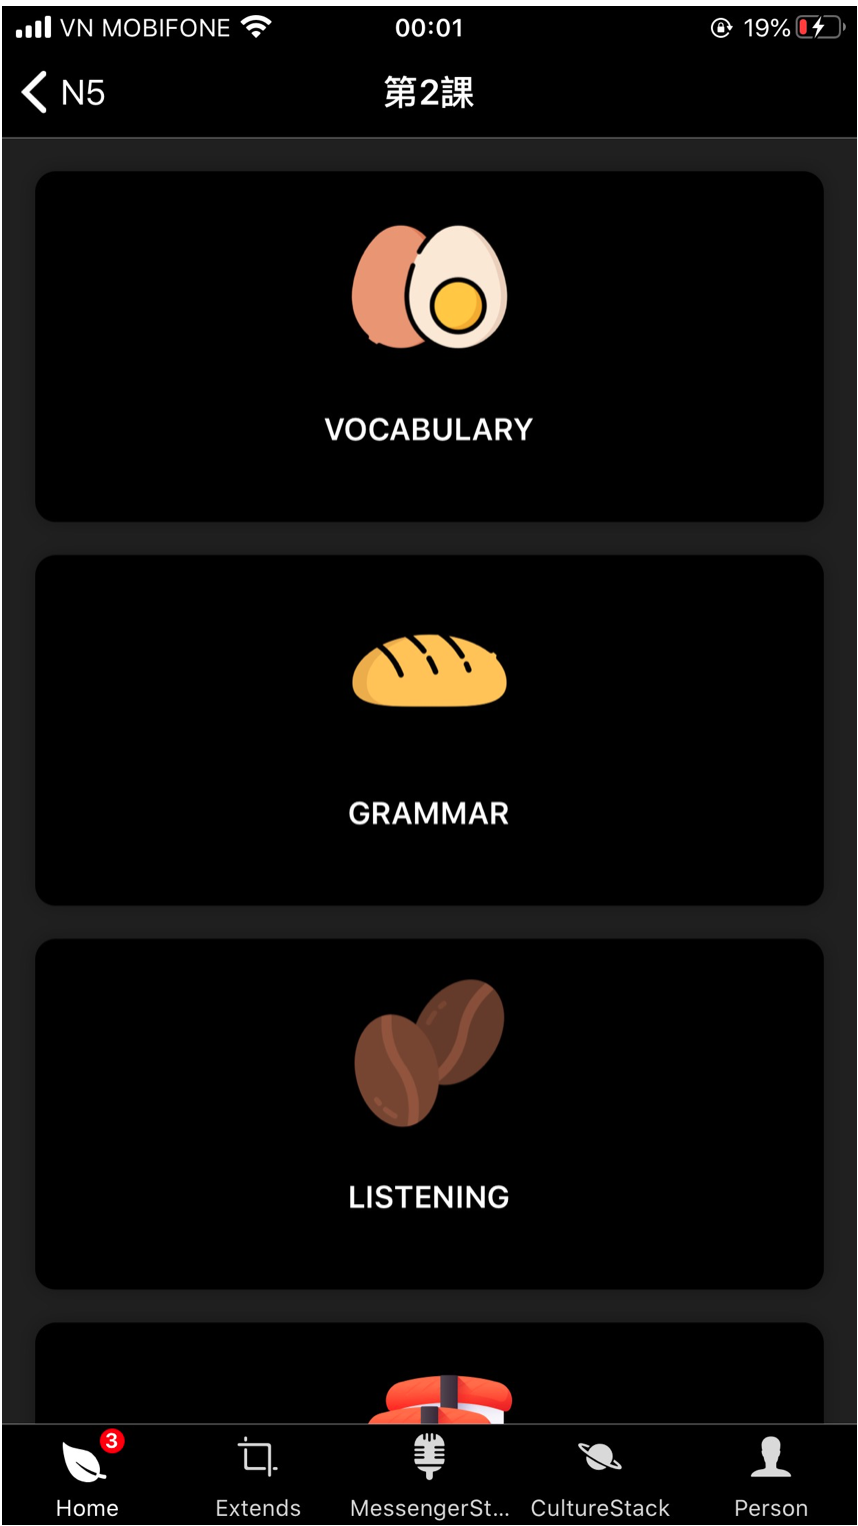
\includegraphics[width=.35\textwidth]{demo-8}
\end{figure}

\end{frame}


\begin{frame}

\centering
Cảm ơn Thầy và các bạn đã chú ý theo dõi và lắng nghe.

\begin{figure}[h]
	\vspace{5pt}
	\centering
	
\includegraphics[width=.9\textwidth]{the-end-6}
\end{figure}
	
\end{frame}

\end{document}